
% Default to the notebook output style

    


% Inherit from the specified cell style.




    
\documentclass[11pt]{article}

    
    
    \usepackage[T1]{fontenc}
    % Nicer default font (+ math font) than Computer Modern for most use cases
    \usepackage{mathpazo}

    % Basic figure setup, for now with no caption control since it's done
    % automatically by Pandoc (which extracts ![](path) syntax from Markdown).
    \usepackage{graphicx}
    % We will generate all images so they have a width \maxwidth. This means
    % that they will get their normal width if they fit onto the page, but
    % are scaled down if they would overflow the margins.
    \makeatletter
    \def\maxwidth{\ifdim\Gin@nat@width>\linewidth\linewidth
    \else\Gin@nat@width\fi}
    \makeatother
    \let\Oldincludegraphics\includegraphics
    % Set max figure width to be 80% of text width, for now hardcoded.
    \renewcommand{\includegraphics}[1]{\Oldincludegraphics[width=.8\maxwidth]{#1}}
    % Ensure that by default, figures have no caption (until we provide a
    % proper Figure object with a Caption API and a way to capture that
    % in the conversion process - todo).
    \usepackage{caption}
    \DeclareCaptionLabelFormat{nolabel}{}
    \captionsetup{labelformat=nolabel}

    \usepackage{adjustbox} % Used to constrain images to a maximum size 
    \usepackage{xcolor} % Allow colors to be defined
    \usepackage{enumerate} % Needed for markdown enumerations to work
    \usepackage{geometry} % Used to adjust the document margins
    \usepackage{amsmath} % Equations
    \usepackage{amssymb} % Equations
    \usepackage{textcomp} % defines textquotesingle
    % Hack from http://tex.stackexchange.com/a/47451/13684:
    \AtBeginDocument{%
        \def\PYZsq{\textquotesingle}% Upright quotes in Pygmentized code
    }
    \usepackage{upquote} % Upright quotes for verbatim code
    \usepackage{eurosym} % defines \euro
    \usepackage[mathletters]{ucs} % Extended unicode (utf-8) support
    \usepackage[utf8x]{inputenc} % Allow utf-8 characters in the tex document
    \usepackage{fancyvrb} % verbatim replacement that allows latex
    \usepackage{grffile} % extends the file name processing of package graphics 
                         % to support a larger range 
    % The hyperref package gives us a pdf with properly built
    % internal navigation ('pdf bookmarks' for the table of contents,
    % internal cross-reference links, web links for URLs, etc.)
    \usepackage{hyperref}
    \usepackage{longtable} % longtable support required by pandoc >1.10
    \usepackage{booktabs}  % table support for pandoc > 1.12.2
    \usepackage[inline]{enumitem} % IRkernel/repr support (it uses the enumerate* environment)
    \usepackage[normalem]{ulem} % ulem is needed to support strikethroughs (\sout)
                                % normalem makes italics be italics, not underlines
    

    
    
    % Colors for the hyperref package
    \definecolor{urlcolor}{rgb}{0,.145,.698}
    \definecolor{linkcolor}{rgb}{.71,0.21,0.01}
    \definecolor{citecolor}{rgb}{.12,.54,.11}

    % ANSI colors
    \definecolor{ansi-black}{HTML}{3E424D}
    \definecolor{ansi-black-intense}{HTML}{282C36}
    \definecolor{ansi-red}{HTML}{E75C58}
    \definecolor{ansi-red-intense}{HTML}{B22B31}
    \definecolor{ansi-green}{HTML}{00A250}
    \definecolor{ansi-green-intense}{HTML}{007427}
    \definecolor{ansi-yellow}{HTML}{DDB62B}
    \definecolor{ansi-yellow-intense}{HTML}{B27D12}
    \definecolor{ansi-blue}{HTML}{208FFB}
    \definecolor{ansi-blue-intense}{HTML}{0065CA}
    \definecolor{ansi-magenta}{HTML}{D160C4}
    \definecolor{ansi-magenta-intense}{HTML}{A03196}
    \definecolor{ansi-cyan}{HTML}{60C6C8}
    \definecolor{ansi-cyan-intense}{HTML}{258F8F}
    \definecolor{ansi-white}{HTML}{C5C1B4}
    \definecolor{ansi-white-intense}{HTML}{A1A6B2}

    % commands and environments needed by pandoc snippets
    % extracted from the output of `pandoc -s`
    \providecommand{\tightlist}{%
      \setlength{\itemsep}{0pt}\setlength{\parskip}{0pt}}
    \DefineVerbatimEnvironment{Highlighting}{Verbatim}{commandchars=\\\{\}}
    % Add ',fontsize=\small' for more characters per line
    \newenvironment{Shaded}{}{}
    \newcommand{\KeywordTok}[1]{\textcolor[rgb]{0.00,0.44,0.13}{\textbf{{#1}}}}
    \newcommand{\DataTypeTok}[1]{\textcolor[rgb]{0.56,0.13,0.00}{{#1}}}
    \newcommand{\DecValTok}[1]{\textcolor[rgb]{0.25,0.63,0.44}{{#1}}}
    \newcommand{\BaseNTok}[1]{\textcolor[rgb]{0.25,0.63,0.44}{{#1}}}
    \newcommand{\FloatTok}[1]{\textcolor[rgb]{0.25,0.63,0.44}{{#1}}}
    \newcommand{\CharTok}[1]{\textcolor[rgb]{0.25,0.44,0.63}{{#1}}}
    \newcommand{\StringTok}[1]{\textcolor[rgb]{0.25,0.44,0.63}{{#1}}}
    \newcommand{\CommentTok}[1]{\textcolor[rgb]{0.38,0.63,0.69}{\textit{{#1}}}}
    \newcommand{\OtherTok}[1]{\textcolor[rgb]{0.00,0.44,0.13}{{#1}}}
    \newcommand{\AlertTok}[1]{\textcolor[rgb]{1.00,0.00,0.00}{\textbf{{#1}}}}
    \newcommand{\FunctionTok}[1]{\textcolor[rgb]{0.02,0.16,0.49}{{#1}}}
    \newcommand{\RegionMarkerTok}[1]{{#1}}
    \newcommand{\ErrorTok}[1]{\textcolor[rgb]{1.00,0.00,0.00}{\textbf{{#1}}}}
    \newcommand{\NormalTok}[1]{{#1}}
    
    % Additional commands for more recent versions of Pandoc
    \newcommand{\ConstantTok}[1]{\textcolor[rgb]{0.53,0.00,0.00}{{#1}}}
    \newcommand{\SpecialCharTok}[1]{\textcolor[rgb]{0.25,0.44,0.63}{{#1}}}
    \newcommand{\VerbatimStringTok}[1]{\textcolor[rgb]{0.25,0.44,0.63}{{#1}}}
    \newcommand{\SpecialStringTok}[1]{\textcolor[rgb]{0.73,0.40,0.53}{{#1}}}
    \newcommand{\ImportTok}[1]{{#1}}
    \newcommand{\DocumentationTok}[1]{\textcolor[rgb]{0.73,0.13,0.13}{\textit{{#1}}}}
    \newcommand{\AnnotationTok}[1]{\textcolor[rgb]{0.38,0.63,0.69}{\textbf{\textit{{#1}}}}}
    \newcommand{\CommentVarTok}[1]{\textcolor[rgb]{0.38,0.63,0.69}{\textbf{\textit{{#1}}}}}
    \newcommand{\VariableTok}[1]{\textcolor[rgb]{0.10,0.09,0.49}{{#1}}}
    \newcommand{\ControlFlowTok}[1]{\textcolor[rgb]{0.00,0.44,0.13}{\textbf{{#1}}}}
    \newcommand{\OperatorTok}[1]{\textcolor[rgb]{0.40,0.40,0.40}{{#1}}}
    \newcommand{\BuiltInTok}[1]{{#1}}
    \newcommand{\ExtensionTok}[1]{{#1}}
    \newcommand{\PreprocessorTok}[1]{\textcolor[rgb]{0.74,0.48,0.00}{{#1}}}
    \newcommand{\AttributeTok}[1]{\textcolor[rgb]{0.49,0.56,0.16}{{#1}}}
    \newcommand{\InformationTok}[1]{\textcolor[rgb]{0.38,0.63,0.69}{\textbf{\textit{{#1}}}}}
    \newcommand{\WarningTok}[1]{\textcolor[rgb]{0.38,0.63,0.69}{\textbf{\textit{{#1}}}}}
    
    
    % Define a nice break command that doesn't care if a line doesn't already
    % exist.
    \def\br{\hspace*{\fill} \\* }
    % Math Jax compatability definitions
    \def\gt{>}
    \def\lt{<}
    % Document parameters
    \title{Exam Task - Spam Message Classifier}
    
    
    

    % Pygments definitions
    
\makeatletter
\def\PY@reset{\let\PY@it=\relax \let\PY@bf=\relax%
    \let\PY@ul=\relax \let\PY@tc=\relax%
    \let\PY@bc=\relax \let\PY@ff=\relax}
\def\PY@tok#1{\csname PY@tok@#1\endcsname}
\def\PY@toks#1+{\ifx\relax#1\empty\else%
    \PY@tok{#1}\expandafter\PY@toks\fi}
\def\PY@do#1{\PY@bc{\PY@tc{\PY@ul{%
    \PY@it{\PY@bf{\PY@ff{#1}}}}}}}
\def\PY#1#2{\PY@reset\PY@toks#1+\relax+\PY@do{#2}}

\expandafter\def\csname PY@tok@w\endcsname{\def\PY@tc##1{\textcolor[rgb]{0.73,0.73,0.73}{##1}}}
\expandafter\def\csname PY@tok@c\endcsname{\let\PY@it=\textit\def\PY@tc##1{\textcolor[rgb]{0.25,0.50,0.50}{##1}}}
\expandafter\def\csname PY@tok@cp\endcsname{\def\PY@tc##1{\textcolor[rgb]{0.74,0.48,0.00}{##1}}}
\expandafter\def\csname PY@tok@k\endcsname{\let\PY@bf=\textbf\def\PY@tc##1{\textcolor[rgb]{0.00,0.50,0.00}{##1}}}
\expandafter\def\csname PY@tok@kp\endcsname{\def\PY@tc##1{\textcolor[rgb]{0.00,0.50,0.00}{##1}}}
\expandafter\def\csname PY@tok@kt\endcsname{\def\PY@tc##1{\textcolor[rgb]{0.69,0.00,0.25}{##1}}}
\expandafter\def\csname PY@tok@o\endcsname{\def\PY@tc##1{\textcolor[rgb]{0.40,0.40,0.40}{##1}}}
\expandafter\def\csname PY@tok@ow\endcsname{\let\PY@bf=\textbf\def\PY@tc##1{\textcolor[rgb]{0.67,0.13,1.00}{##1}}}
\expandafter\def\csname PY@tok@nb\endcsname{\def\PY@tc##1{\textcolor[rgb]{0.00,0.50,0.00}{##1}}}
\expandafter\def\csname PY@tok@nf\endcsname{\def\PY@tc##1{\textcolor[rgb]{0.00,0.00,1.00}{##1}}}
\expandafter\def\csname PY@tok@nc\endcsname{\let\PY@bf=\textbf\def\PY@tc##1{\textcolor[rgb]{0.00,0.00,1.00}{##1}}}
\expandafter\def\csname PY@tok@nn\endcsname{\let\PY@bf=\textbf\def\PY@tc##1{\textcolor[rgb]{0.00,0.00,1.00}{##1}}}
\expandafter\def\csname PY@tok@ne\endcsname{\let\PY@bf=\textbf\def\PY@tc##1{\textcolor[rgb]{0.82,0.25,0.23}{##1}}}
\expandafter\def\csname PY@tok@nv\endcsname{\def\PY@tc##1{\textcolor[rgb]{0.10,0.09,0.49}{##1}}}
\expandafter\def\csname PY@tok@no\endcsname{\def\PY@tc##1{\textcolor[rgb]{0.53,0.00,0.00}{##1}}}
\expandafter\def\csname PY@tok@nl\endcsname{\def\PY@tc##1{\textcolor[rgb]{0.63,0.63,0.00}{##1}}}
\expandafter\def\csname PY@tok@ni\endcsname{\let\PY@bf=\textbf\def\PY@tc##1{\textcolor[rgb]{0.60,0.60,0.60}{##1}}}
\expandafter\def\csname PY@tok@na\endcsname{\def\PY@tc##1{\textcolor[rgb]{0.49,0.56,0.16}{##1}}}
\expandafter\def\csname PY@tok@nt\endcsname{\let\PY@bf=\textbf\def\PY@tc##1{\textcolor[rgb]{0.00,0.50,0.00}{##1}}}
\expandafter\def\csname PY@tok@nd\endcsname{\def\PY@tc##1{\textcolor[rgb]{0.67,0.13,1.00}{##1}}}
\expandafter\def\csname PY@tok@s\endcsname{\def\PY@tc##1{\textcolor[rgb]{0.73,0.13,0.13}{##1}}}
\expandafter\def\csname PY@tok@sd\endcsname{\let\PY@it=\textit\def\PY@tc##1{\textcolor[rgb]{0.73,0.13,0.13}{##1}}}
\expandafter\def\csname PY@tok@si\endcsname{\let\PY@bf=\textbf\def\PY@tc##1{\textcolor[rgb]{0.73,0.40,0.53}{##1}}}
\expandafter\def\csname PY@tok@se\endcsname{\let\PY@bf=\textbf\def\PY@tc##1{\textcolor[rgb]{0.73,0.40,0.13}{##1}}}
\expandafter\def\csname PY@tok@sr\endcsname{\def\PY@tc##1{\textcolor[rgb]{0.73,0.40,0.53}{##1}}}
\expandafter\def\csname PY@tok@ss\endcsname{\def\PY@tc##1{\textcolor[rgb]{0.10,0.09,0.49}{##1}}}
\expandafter\def\csname PY@tok@sx\endcsname{\def\PY@tc##1{\textcolor[rgb]{0.00,0.50,0.00}{##1}}}
\expandafter\def\csname PY@tok@m\endcsname{\def\PY@tc##1{\textcolor[rgb]{0.40,0.40,0.40}{##1}}}
\expandafter\def\csname PY@tok@gh\endcsname{\let\PY@bf=\textbf\def\PY@tc##1{\textcolor[rgb]{0.00,0.00,0.50}{##1}}}
\expandafter\def\csname PY@tok@gu\endcsname{\let\PY@bf=\textbf\def\PY@tc##1{\textcolor[rgb]{0.50,0.00,0.50}{##1}}}
\expandafter\def\csname PY@tok@gd\endcsname{\def\PY@tc##1{\textcolor[rgb]{0.63,0.00,0.00}{##1}}}
\expandafter\def\csname PY@tok@gi\endcsname{\def\PY@tc##1{\textcolor[rgb]{0.00,0.63,0.00}{##1}}}
\expandafter\def\csname PY@tok@gr\endcsname{\def\PY@tc##1{\textcolor[rgb]{1.00,0.00,0.00}{##1}}}
\expandafter\def\csname PY@tok@ge\endcsname{\let\PY@it=\textit}
\expandafter\def\csname PY@tok@gs\endcsname{\let\PY@bf=\textbf}
\expandafter\def\csname PY@tok@gp\endcsname{\let\PY@bf=\textbf\def\PY@tc##1{\textcolor[rgb]{0.00,0.00,0.50}{##1}}}
\expandafter\def\csname PY@tok@go\endcsname{\def\PY@tc##1{\textcolor[rgb]{0.53,0.53,0.53}{##1}}}
\expandafter\def\csname PY@tok@gt\endcsname{\def\PY@tc##1{\textcolor[rgb]{0.00,0.27,0.87}{##1}}}
\expandafter\def\csname PY@tok@err\endcsname{\def\PY@bc##1{\setlength{\fboxsep}{0pt}\fcolorbox[rgb]{1.00,0.00,0.00}{1,1,1}{\strut ##1}}}
\expandafter\def\csname PY@tok@kc\endcsname{\let\PY@bf=\textbf\def\PY@tc##1{\textcolor[rgb]{0.00,0.50,0.00}{##1}}}
\expandafter\def\csname PY@tok@kd\endcsname{\let\PY@bf=\textbf\def\PY@tc##1{\textcolor[rgb]{0.00,0.50,0.00}{##1}}}
\expandafter\def\csname PY@tok@kn\endcsname{\let\PY@bf=\textbf\def\PY@tc##1{\textcolor[rgb]{0.00,0.50,0.00}{##1}}}
\expandafter\def\csname PY@tok@kr\endcsname{\let\PY@bf=\textbf\def\PY@tc##1{\textcolor[rgb]{0.00,0.50,0.00}{##1}}}
\expandafter\def\csname PY@tok@bp\endcsname{\def\PY@tc##1{\textcolor[rgb]{0.00,0.50,0.00}{##1}}}
\expandafter\def\csname PY@tok@fm\endcsname{\def\PY@tc##1{\textcolor[rgb]{0.00,0.00,1.00}{##1}}}
\expandafter\def\csname PY@tok@vc\endcsname{\def\PY@tc##1{\textcolor[rgb]{0.10,0.09,0.49}{##1}}}
\expandafter\def\csname PY@tok@vg\endcsname{\def\PY@tc##1{\textcolor[rgb]{0.10,0.09,0.49}{##1}}}
\expandafter\def\csname PY@tok@vi\endcsname{\def\PY@tc##1{\textcolor[rgb]{0.10,0.09,0.49}{##1}}}
\expandafter\def\csname PY@tok@vm\endcsname{\def\PY@tc##1{\textcolor[rgb]{0.10,0.09,0.49}{##1}}}
\expandafter\def\csname PY@tok@sa\endcsname{\def\PY@tc##1{\textcolor[rgb]{0.73,0.13,0.13}{##1}}}
\expandafter\def\csname PY@tok@sb\endcsname{\def\PY@tc##1{\textcolor[rgb]{0.73,0.13,0.13}{##1}}}
\expandafter\def\csname PY@tok@sc\endcsname{\def\PY@tc##1{\textcolor[rgb]{0.73,0.13,0.13}{##1}}}
\expandafter\def\csname PY@tok@dl\endcsname{\def\PY@tc##1{\textcolor[rgb]{0.73,0.13,0.13}{##1}}}
\expandafter\def\csname PY@tok@s2\endcsname{\def\PY@tc##1{\textcolor[rgb]{0.73,0.13,0.13}{##1}}}
\expandafter\def\csname PY@tok@sh\endcsname{\def\PY@tc##1{\textcolor[rgb]{0.73,0.13,0.13}{##1}}}
\expandafter\def\csname PY@tok@s1\endcsname{\def\PY@tc##1{\textcolor[rgb]{0.73,0.13,0.13}{##1}}}
\expandafter\def\csname PY@tok@mb\endcsname{\def\PY@tc##1{\textcolor[rgb]{0.40,0.40,0.40}{##1}}}
\expandafter\def\csname PY@tok@mf\endcsname{\def\PY@tc##1{\textcolor[rgb]{0.40,0.40,0.40}{##1}}}
\expandafter\def\csname PY@tok@mh\endcsname{\def\PY@tc##1{\textcolor[rgb]{0.40,0.40,0.40}{##1}}}
\expandafter\def\csname PY@tok@mi\endcsname{\def\PY@tc##1{\textcolor[rgb]{0.40,0.40,0.40}{##1}}}
\expandafter\def\csname PY@tok@il\endcsname{\def\PY@tc##1{\textcolor[rgb]{0.40,0.40,0.40}{##1}}}
\expandafter\def\csname PY@tok@mo\endcsname{\def\PY@tc##1{\textcolor[rgb]{0.40,0.40,0.40}{##1}}}
\expandafter\def\csname PY@tok@ch\endcsname{\let\PY@it=\textit\def\PY@tc##1{\textcolor[rgb]{0.25,0.50,0.50}{##1}}}
\expandafter\def\csname PY@tok@cm\endcsname{\let\PY@it=\textit\def\PY@tc##1{\textcolor[rgb]{0.25,0.50,0.50}{##1}}}
\expandafter\def\csname PY@tok@cpf\endcsname{\let\PY@it=\textit\def\PY@tc##1{\textcolor[rgb]{0.25,0.50,0.50}{##1}}}
\expandafter\def\csname PY@tok@c1\endcsname{\let\PY@it=\textit\def\PY@tc##1{\textcolor[rgb]{0.25,0.50,0.50}{##1}}}
\expandafter\def\csname PY@tok@cs\endcsname{\let\PY@it=\textit\def\PY@tc##1{\textcolor[rgb]{0.25,0.50,0.50}{##1}}}

\def\PYZbs{\char`\\}
\def\PYZus{\char`\_}
\def\PYZob{\char`\{}
\def\PYZcb{\char`\}}
\def\PYZca{\char`\^}
\def\PYZam{\char`\&}
\def\PYZlt{\char`\<}
\def\PYZgt{\char`\>}
\def\PYZsh{\char`\#}
\def\PYZpc{\char`\%}
\def\PYZdl{\char`\$}
\def\PYZhy{\char`\-}
\def\PYZsq{\char`\'}
\def\PYZdq{\char`\"}
\def\PYZti{\char`\~}
% for compatibility with earlier versions
\def\PYZat{@}
\def\PYZlb{[}
\def\PYZrb{]}
\makeatother


    % Exact colors from NB
    \definecolor{incolor}{rgb}{0.0, 0.0, 0.5}
    \definecolor{outcolor}{rgb}{0.545, 0.0, 0.0}



    
    % Prevent overflowing lines due to hard-to-break entities
    \sloppy 
    % Setup hyperref package
    \hypersetup{
      breaklinks=true,  % so long urls are correctly broken across lines
      colorlinks=true,
      urlcolor=urlcolor,
      linkcolor=linkcolor,
      citecolor=citecolor,
      }
    % Slightly bigger margins than the latex defaults
    
    \geometry{verbose,tmargin=1in,bmargin=1in,lmargin=1in,rmargin=1in}
    
    

    \begin{document}
    
    
    \maketitle
    
    

    
    \section{SPAM message classifier}\label{spam-message-classifier}

    This task is based on the spam message dataset provided at
http://www.dt.fee.unicamp.br/\textasciitilde{}tiago/smsspamcollection/ .
"The SMS Spam Collection is a set of SMS tagged messages that have been
collected for SMS Spam research. It contains one set of SMS messages in
English of 5,574 messages, tagged acording being ham (legitimate) or
spam."

The data is being used to train a couple of our models as well check the
accuracy of prediction. Then we this model will be integrated into our
simple web application where you can input a text string get prediction
results, if the message is indeed a spam.

    \subsection{1. Import and manipulate/check
data}\label{import-and-manipulatecheck-data}

    \begin{Verbatim}[commandchars=\\\{\}]
{\color{incolor}In [{\color{incolor}1}]:} \PY{k+kn}{import} \PY{n+nn}{pandas} \PY{k}{as} \PY{n+nn}{pd}
        \PY{k+kn}{import} \PY{n+nn}{numpy} \PY{k}{as} \PY{n+nn}{np}
        \PY{k+kn}{import} \PY{n+nn}{matplotlib}\PY{n+nn}{.}\PY{n+nn}{pyplot} \PY{k}{as} \PY{n+nn}{plt}
        \PY{k+kn}{import} \PY{n+nn}{seaborn} \PY{k}{as} \PY{n+nn}{sns}
        \PY{o}{\PYZpc{}}\PY{k}{matplotlib} inline
\end{Verbatim}


    \begin{Verbatim}[commandchars=\\\{\}]
{\color{incolor}In [{\color{incolor}2}]:} \PY{c+c1}{\PYZsh{} load data from csv file}
        \PY{n}{data} \PY{o}{=} \PY{n}{pd}\PY{o}{.}\PY{n}{read\PYZus{}csv}\PY{p}{(}\PY{l+s+s2}{\PYZdq{}}\PY{l+s+s2}{./data/spam.csv}\PY{l+s+s2}{\PYZdq{}}\PY{p}{,}\PY{n}{encoding}\PY{o}{=}\PY{l+s+s1}{\PYZsq{}}\PY{l+s+s1}{latin\PYZhy{}1}\PY{l+s+s1}{\PYZsq{}}\PY{p}{)}
\end{Verbatim}


    \begin{Verbatim}[commandchars=\\\{\}]
{\color{incolor}In [{\color{incolor}3}]:} \PY{n}{data}\PY{o}{.}\PY{n}{shape}
\end{Verbatim}


\begin{Verbatim}[commandchars=\\\{\}]
{\color{outcolor}Out[{\color{outcolor}3}]:} (5572, 5)
\end{Verbatim}
            
    \begin{Verbatim}[commandchars=\\\{\}]
{\color{incolor}In [{\color{incolor}4}]:} \PY{n}{data}\PY{o}{.}\PY{n}{head}\PY{p}{(}\PY{l+m+mi}{5}\PY{p}{)}
\end{Verbatim}


\begin{Verbatim}[commandchars=\\\{\}]
{\color{outcolor}Out[{\color{outcolor}4}]:}      v1                                                 v2 Unnamed: 2  \textbackslash{}
        0   ham  Go until jurong point, crazy.. Available only {\ldots}        NaN   
        1   ham                      Ok lar{\ldots} Joking wif u oni{\ldots}        NaN   
        2  spam  Free entry in 2 a wkly comp to win FA Cup fina{\ldots}        NaN   
        3   ham  U dun say so early hor{\ldots} U c already then say{\ldots}        NaN   
        4   ham  Nah I don't think he goes to usf, he lives aro{\ldots}        NaN   
        
          Unnamed: 3 Unnamed: 4  
        0        NaN        NaN  
        1        NaN        NaN  
        2        NaN        NaN  
        3        NaN        NaN  
        4        NaN        NaN  
\end{Verbatim}
            
    \begin{Verbatim}[commandchars=\\\{\}]
{\color{incolor}In [{\color{incolor}5}]:} \PY{c+c1}{\PYZsh{} select and rename the columns relevant to us }
        \PY{n}{data} \PY{o}{=} \PY{n}{data}\PY{p}{[}\PY{p}{[}\PY{l+s+s1}{\PYZsq{}}\PY{l+s+s1}{v2}\PY{l+s+s1}{\PYZsq{}}\PY{p}{,}\PY{l+s+s1}{\PYZsq{}}\PY{l+s+s1}{v1}\PY{l+s+s1}{\PYZsq{}}\PY{p}{]}\PY{p}{]}
        \PY{n}{data} \PY{o}{=} \PY{n}{data}\PY{o}{.}\PY{n}{rename}\PY{p}{(}\PY{n}{columns}\PY{o}{=}\PY{p}{\PYZob{}}\PY{l+s+s2}{\PYZdq{}}\PY{l+s+s2}{v1}\PY{l+s+s2}{\PYZdq{}}\PY{p}{:}\PY{l+s+s2}{\PYZdq{}}\PY{l+s+s2}{label}\PY{l+s+s2}{\PYZdq{}}\PY{p}{,} \PY{l+s+s2}{\PYZdq{}}\PY{l+s+s2}{v2}\PY{l+s+s2}{\PYZdq{}}\PY{p}{:}\PY{l+s+s2}{\PYZdq{}}\PY{l+s+s2}{text}\PY{l+s+s2}{\PYZdq{}}\PY{p}{\PYZcb{}}\PY{p}{)}
        
        \PY{n+nb}{print}\PY{p}{(}\PY{n}{data}\PY{o}{.}\PY{n}{groupby}\PY{p}{(}\PY{l+s+s1}{\PYZsq{}}\PY{l+s+s1}{label}\PY{l+s+s1}{\PYZsq{}}\PY{p}{)}\PY{o}{.}\PY{n}{size}\PY{p}{(}\PY{p}{)}\PY{p}{)}
\end{Verbatim}


    \begin{Verbatim}[commandchars=\\\{\}]
label
ham     4825
spam     747
dtype: int64

    \end{Verbatim}

    \begin{Verbatim}[commandchars=\\\{\}]
{\color{incolor}In [{\color{incolor}6}]:} \PY{n}{data}\PY{o}{.}\PY{n}{isnull}\PY{p}{(}\PY{p}{)}\PY{o}{.}\PY{n}{values}\PY{o}{.}\PY{n}{any}\PY{p}{(}\PY{p}{)}
\end{Verbatim}


\begin{Verbatim}[commandchars=\\\{\}]
{\color{outcolor}Out[{\color{outcolor}6}]:} False
\end{Verbatim}
            
    \begin{Verbatim}[commandchars=\\\{\}]
{\color{incolor}In [{\color{incolor}7}]:} \PY{c+c1}{\PYZsh{} convert the output data/ label to binary value}
        \PY{n}{data}\PY{p}{[}\PY{l+s+s1}{\PYZsq{}}\PY{l+s+s1}{label}\PY{l+s+s1}{\PYZsq{}}\PY{p}{]} \PY{o}{=} \PY{n}{data}\PY{o}{.}\PY{n}{label}\PY{o}{.}\PY{n}{replace}\PY{p}{(}\PY{n}{to\PYZus{}replace}\PY{o}{=}\PY{p}{[}\PY{l+s+s1}{\PYZsq{}}\PY{l+s+s1}{ham}\PY{l+s+s1}{\PYZsq{}}\PY{p}{,} \PY{l+s+s1}{\PYZsq{}}\PY{l+s+s1}{spam}\PY{l+s+s1}{\PYZsq{}}\PY{p}{]}\PY{p}{,} \PY{n}{value}\PY{o}{=}\PY{p}{[}\PY{l+m+mi}{0}\PY{p}{,} \PY{l+m+mi}{1}\PY{p}{]}\PY{p}{)}
\end{Verbatim}


    \begin{Verbatim}[commandchars=\\\{\}]
{\color{incolor}In [{\color{incolor}8}]:} \PY{n}{data}\PY{o}{.}\PY{n}{head}\PY{p}{(}\PY{l+m+mi}{5}\PY{p}{)}
\end{Verbatim}


\begin{Verbatim}[commandchars=\\\{\}]
{\color{outcolor}Out[{\color{outcolor}8}]:}                                                 text  label
        0  Go until jurong point, crazy.. Available only {\ldots}      0
        1                      Ok lar{\ldots} Joking wif u oni{\ldots}      0
        2  Free entry in 2 a wkly comp to win FA Cup fina{\ldots}      1
        3  U dun say so early hor{\ldots} U c already then say{\ldots}      0
        4  Nah I don't think he goes to usf, he lives aro{\ldots}      0
\end{Verbatim}
            
    \subsection{2. Visualization of data}\label{visualization-of-data}

    We used a visualization example for wordcloud to get an overview of the
words present in the spam and legitimate messages

    \subsubsection{2.1 Message length distribution per
category}\label{message-length-distribution-per-category}

    \begin{Verbatim}[commandchars=\\\{\}]
{\color{incolor}In [{\color{incolor}9}]:} \PY{n}{plotdata} \PY{o}{=} \PY{n}{data}
        \PY{n}{plotdata}\PY{p}{[}\PY{l+s+s2}{\PYZdq{}}\PY{l+s+s2}{message\PYZus{}length}\PY{l+s+s2}{\PYZdq{}}\PY{p}{]} \PY{o}{=} \PY{n}{data}\PY{p}{[}\PY{l+s+s2}{\PYZdq{}}\PY{l+s+s2}{text}\PY{l+s+s2}{\PYZdq{}}\PY{p}{]}\PY{o}{.}\PY{n}{apply}\PY{p}{(}\PY{n+nb}{len}\PY{p}{)}
        
        \PY{n}{f}\PY{p}{,} \PY{n}{ax} \PY{o}{=} \PY{n}{plt}\PY{o}{.}\PY{n}{subplots}\PY{p}{(}\PY{l+m+mi}{1}\PY{p}{,} \PY{l+m+mi}{2}\PY{p}{,} \PY{n}{figsize} \PY{o}{=} \PY{p}{(}\PY{l+m+mi}{20}\PY{p}{,} \PY{l+m+mi}{6}\PY{p}{)}\PY{p}{)}
        
        
        \PY{n}{sns}\PY{o}{.}\PY{n}{distplot}\PY{p}{(}\PY{n}{plotdata}\PY{p}{[}\PY{n}{plotdata}\PY{p}{[}\PY{l+s+s2}{\PYZdq{}}\PY{l+s+s2}{label}\PY{l+s+s2}{\PYZdq{}}\PY{p}{]} \PY{o}{==} \PY{l+m+mi}{1}\PY{p}{]}\PY{p}{[}\PY{l+s+s2}{\PYZdq{}}\PY{l+s+s2}{message\PYZus{}length}\PY{l+s+s2}{\PYZdq{}}\PY{p}{]}\PY{p}{,} \PY{n}{bins} \PY{o}{=} \PY{l+m+mi}{20}\PY{p}{,} \PY{n}{ax} \PY{o}{=} \PY{n}{ax}\PY{p}{[}\PY{l+m+mi}{0}\PY{p}{]}\PY{p}{)}
        \PY{n}{ax}\PY{p}{[}\PY{l+m+mi}{0}\PY{p}{]}\PY{o}{.}\PY{n}{set\PYZus{}xlabel}\PY{p}{(}\PY{l+s+s2}{\PYZdq{}}\PY{l+s+s2}{Spam Message Word Length}\PY{l+s+s2}{\PYZdq{}}\PY{p}{)}
        
        \PY{n}{sns}\PY{o}{.}\PY{n}{distplot}\PY{p}{(}\PY{n}{plotdata}\PY{p}{[}\PY{n}{plotdata}\PY{p}{[}\PY{l+s+s2}{\PYZdq{}}\PY{l+s+s2}{label}\PY{l+s+s2}{\PYZdq{}}\PY{p}{]}\PY{o}{==} \PY{l+m+mi}{0}\PY{p}{]}\PY{p}{[}\PY{l+s+s2}{\PYZdq{}}\PY{l+s+s2}{message\PYZus{}length}\PY{l+s+s2}{\PYZdq{}}\PY{p}{]}\PY{p}{,} \PY{n}{bins} \PY{o}{=} \PY{l+m+mi}{20}\PY{p}{,} \PY{n}{ax} \PY{o}{=} \PY{n}{ax}\PY{p}{[}\PY{l+m+mi}{1}\PY{p}{]}\PY{p}{)}
        \PY{n}{ax}\PY{p}{[}\PY{l+m+mi}{0}\PY{p}{]}\PY{o}{.}\PY{n}{set\PYZus{}xlabel}\PY{p}{(}\PY{l+s+s2}{\PYZdq{}}\PY{l+s+s2}{Ham Message Word Length}\PY{l+s+s2}{\PYZdq{}}\PY{p}{)}
        
        \PY{n}{plt}\PY{o}{.}\PY{n}{show}\PY{p}{(}\PY{p}{)}
\end{Verbatim}


    \begin{Verbatim}[commandchars=\\\{\}]
C:\textbackslash{}ProgramData\textbackslash{}Anaconda3\textbackslash{}lib\textbackslash{}site-packages\textbackslash{}matplotlib\textbackslash{}axes\textbackslash{}\_axes.py:6462: UserWarning: The 'normed' kwarg is deprecated, and has been replaced by the 'density' kwarg.
  warnings.warn("The 'normed' kwarg is deprecated, and has been "
C:\textbackslash{}ProgramData\textbackslash{}Anaconda3\textbackslash{}lib\textbackslash{}site-packages\textbackslash{}matplotlib\textbackslash{}axes\textbackslash{}\_axes.py:6462: UserWarning: The 'normed' kwarg is deprecated, and has been replaced by the 'density' kwarg.
  warnings.warn("The 'normed' kwarg is deprecated, and has been "

    \end{Verbatim}

    \begin{center}
    \adjustimage{max size={0.9\linewidth}{0.9\paperheight}}{output_14_1.png}
    \end{center}
    { \hspace*{\fill} \\}
    
    \subsubsection{2.2 Word Cloud}\label{word-cloud}

    \begin{Verbatim}[commandchars=\\\{\}]
{\color{incolor}In [{\color{incolor}10}]:} \PY{n}{ham\PYZus{}words} \PY{o}{=} \PY{l+s+s1}{\PYZsq{}}\PY{l+s+s1}{\PYZsq{}}
         \PY{n}{spam\PYZus{}words} \PY{o}{=} \PY{l+s+s1}{\PYZsq{}}\PY{l+s+s1}{\PYZsq{}}
         \PY{n}{spam} \PY{o}{=} \PY{n}{data}\PY{p}{[}\PY{n}{data}\PY{o}{.}\PY{n}{label} \PY{o}{==} \PY{l+m+mi}{1}\PY{p}{]}
         \PY{n}{ham} \PY{o}{=} \PY{n}{data}\PY{p}{[}\PY{n}{data}\PY{o}{.}\PY{n}{label} \PY{o}{==}\PY{l+m+mi}{0}\PY{p}{]}
\end{Verbatim}


    \begin{Verbatim}[commandchars=\\\{\}]
{\color{incolor}In [{\color{incolor}11}]:} \PY{k+kn}{import} \PY{n+nn}{nltk}
\end{Verbatim}


    \begin{Verbatim}[commandchars=\\\{\}]
{\color{incolor}In [{\color{incolor}12}]:} \PY{k}{for} \PY{n}{val} \PY{o+ow}{in} \PY{n}{spam}\PY{o}{.}\PY{n}{text}\PY{p}{:}
             \PY{n}{text} \PY{o}{=} \PY{n}{val}\PY{o}{.}\PY{n}{lower}\PY{p}{(}\PY{p}{)}
             \PY{n}{tokens} \PY{o}{=} \PY{n}{nltk}\PY{o}{.}\PY{n}{word\PYZus{}tokenize}\PY{p}{(}\PY{n}{text}\PY{p}{)}
             \PY{k}{for} \PY{n}{words} \PY{o+ow}{in} \PY{n}{tokens}\PY{p}{:}
                 \PY{n}{spam\PYZus{}words} \PY{o}{=} \PY{n}{spam\PYZus{}words} \PY{o}{+} \PY{n}{words} \PY{o}{+} \PY{l+s+s1}{\PYZsq{}}\PY{l+s+s1}{ }\PY{l+s+s1}{\PYZsq{}}
                 
         \PY{k}{for} \PY{n}{val} \PY{o+ow}{in} \PY{n}{ham}\PY{o}{.}\PY{n}{text}\PY{p}{:}
             \PY{n}{text} \PY{o}{=} \PY{n}{val}\PY{o}{.}\PY{n}{lower}\PY{p}{(}\PY{p}{)}
             \PY{n}{tokens} \PY{o}{=} \PY{n}{nltk}\PY{o}{.}\PY{n}{word\PYZus{}tokenize}\PY{p}{(}\PY{n}{text}\PY{p}{)}
             \PY{k}{for} \PY{n}{words} \PY{o+ow}{in} \PY{n}{tokens}\PY{p}{:}
                 \PY{n}{ham\PYZus{}words} \PY{o}{=} \PY{n}{ham\PYZus{}words} \PY{o}{+} \PY{n}{words} \PY{o}{+} \PY{l+s+s1}{\PYZsq{}}\PY{l+s+s1}{ }\PY{l+s+s1}{\PYZsq{}}
\end{Verbatim}


    \begin{Verbatim}[commandchars=\\\{\}]
{\color{incolor}In [{\color{incolor}13}]:} \PY{k+kn}{from} \PY{n+nn}{wordcloud} \PY{k}{import} \PY{n}{WordCloud}
\end{Verbatim}


    \begin{Verbatim}[commandchars=\\\{\}]
{\color{incolor}In [{\color{incolor}14}]:} \PY{n}{spam\PYZus{}wordcloud} \PY{o}{=} \PY{n}{WordCloud}\PY{p}{(}\PY{n}{width}\PY{o}{=}\PY{l+m+mi}{600}\PY{p}{,} \PY{n}{height}\PY{o}{=}\PY{l+m+mi}{400}\PY{p}{)}\PY{o}{.}\PY{n}{generate}\PY{p}{(}\PY{n}{spam\PYZus{}words}\PY{p}{)}
         \PY{n}{ham\PYZus{}wordcloud} \PY{o}{=} \PY{n}{WordCloud}\PY{p}{(}\PY{n}{width}\PY{o}{=}\PY{l+m+mi}{600}\PY{p}{,} \PY{n}{height}\PY{o}{=}\PY{l+m+mi}{400}\PY{p}{)}\PY{o}{.}\PY{n}{generate}\PY{p}{(}\PY{n}{ham\PYZus{}words}\PY{p}{)}
\end{Verbatim}


    \begin{Verbatim}[commandchars=\\\{\}]
{\color{incolor}In [{\color{incolor}15}]:} \PY{c+c1}{\PYZsh{}Spam Word cloud}
         \PY{n}{plt}\PY{o}{.}\PY{n}{figure}\PY{p}{(} \PY{n}{figsize}\PY{o}{=}\PY{p}{(}\PY{l+m+mi}{10}\PY{p}{,}\PY{l+m+mi}{8}\PY{p}{)}\PY{p}{,} \PY{n}{facecolor}\PY{o}{=}\PY{l+s+s1}{\PYZsq{}}\PY{l+s+s1}{k}\PY{l+s+s1}{\PYZsq{}}\PY{p}{)}
         \PY{n}{plt}\PY{o}{.}\PY{n}{imshow}\PY{p}{(}\PY{n}{spam\PYZus{}wordcloud}\PY{p}{)}
         \PY{n}{plt}\PY{o}{.}\PY{n}{axis}\PY{p}{(}\PY{l+s+s2}{\PYZdq{}}\PY{l+s+s2}{off}\PY{l+s+s2}{\PYZdq{}}\PY{p}{)}
         \PY{n}{plt}\PY{o}{.}\PY{n}{tight\PYZus{}layout}\PY{p}{(}\PY{n}{pad}\PY{o}{=}\PY{l+m+mi}{0}\PY{p}{)}
         \PY{n}{plt}\PY{o}{.}\PY{n}{show}\PY{p}{(}\PY{p}{)}
\end{Verbatim}


    \begin{center}
    \adjustimage{max size={0.9\linewidth}{0.9\paperheight}}{output_21_0.png}
    \end{center}
    { \hspace*{\fill} \\}
    
    \begin{Verbatim}[commandchars=\\\{\}]
{\color{incolor}In [{\color{incolor}16}]:} \PY{c+c1}{\PYZsh{}legitimate/ham word cloud}
         \PY{n}{plt}\PY{o}{.}\PY{n}{figure}\PY{p}{(} \PY{n}{figsize}\PY{o}{=}\PY{p}{(}\PY{l+m+mi}{10}\PY{p}{,}\PY{l+m+mi}{8}\PY{p}{)}\PY{p}{,} \PY{n}{facecolor}\PY{o}{=}\PY{l+s+s1}{\PYZsq{}}\PY{l+s+s1}{k}\PY{l+s+s1}{\PYZsq{}}\PY{p}{)}
         \PY{n}{plt}\PY{o}{.}\PY{n}{imshow}\PY{p}{(}\PY{n}{ham\PYZus{}wordcloud}\PY{p}{)}
         \PY{n}{plt}\PY{o}{.}\PY{n}{axis}\PY{p}{(}\PY{l+s+s2}{\PYZdq{}}\PY{l+s+s2}{off}\PY{l+s+s2}{\PYZdq{}}\PY{p}{)}
         \PY{n}{plt}\PY{o}{.}\PY{n}{tight\PYZus{}layout}\PY{p}{(}\PY{n}{pad}\PY{o}{=}\PY{l+m+mi}{0}\PY{p}{)}
         \PY{n}{plt}\PY{o}{.}\PY{n}{show}\PY{p}{(}\PY{p}{)}
\end{Verbatim}


    \begin{center}
    \adjustimage{max size={0.9\linewidth}{0.9\paperheight}}{output_22_0.png}
    \end{center}
    { \hspace*{\fill} \\}
    
    \subsection{3. Stemming the text
messages}\label{stemming-the-text-messages}

    We are using the nltk module to create corpus (removing special
characters and punctuation) from the text messages and convert the text
to lowercase. Then the stopwords (most common words) are filtered out
and stemming (converting words to thier stem/base word) is performed.
The stemming makes the text dense and reduces the size of dictionary and
takes different variations of words as one. This might sometimes reduces
the accuracy of prediction due to different meaing between the form of
words.

    \begin{Verbatim}[commandchars=\\\{\}]
{\color{incolor}In [{\color{incolor}17}]:} \PY{k+kn}{import} \PY{n+nn}{re}
         \PY{k+kn}{import} \PY{n+nn}{os}
         \PY{k+kn}{from} \PY{n+nn}{nltk}\PY{n+nn}{.}\PY{n+nn}{corpus} \PY{k}{import} \PY{n}{stopwords}
         \PY{k+kn}{from} \PY{n+nn}{nltk}\PY{n+nn}{.}\PY{n+nn}{stem}\PY{n+nn}{.}\PY{n+nn}{porter} \PY{k}{import} \PY{n}{PorterStemmer}
\end{Verbatim}


    \begin{Verbatim}[commandchars=\\\{\}]
{\color{incolor}In [{\color{incolor}18}]:} \PY{n}{portstemmer} \PY{o}{=} \PY{n}{PorterStemmer}\PY{p}{(}\PY{p}{)}
         \PY{n}{stop} \PY{o}{=} \PY{n}{stopwords}\PY{o}{.}\PY{n}{words}\PY{p}{(}\PY{l+s+s1}{\PYZsq{}}\PY{l+s+s1}{english}\PY{l+s+s1}{\PYZsq{}}\PY{p}{)}
         \PY{n}{corpus} \PY{o}{=} \PY{p}{[}\PY{p}{]}
         \PY{k}{for} \PY{n}{i} \PY{o+ow}{in} \PY{n+nb}{range} \PY{p}{(}\PY{l+m+mi}{0}\PY{p}{,}\PY{n+nb}{len}\PY{p}{(}\PY{n}{data}\PY{p}{)}\PY{p}{)}\PY{p}{:}
             \PY{n}{mess} \PY{o}{=} \PY{n}{re}\PY{o}{.}\PY{n}{sub}\PY{p}{(}\PY{l+s+s1}{\PYZsq{}}\PY{l+s+s1}{[\PYZca{}a\PYZhy{}zA\PYZhy{}Z]}\PY{l+s+s1}{\PYZsq{}}\PY{p}{,}\PY{n}{repl} \PY{o}{=} \PY{l+s+s1}{\PYZsq{}}\PY{l+s+s1}{ }\PY{l+s+s1}{\PYZsq{}}\PY{p}{,}\PY{n}{string} \PY{o}{=} \PY{n}{data}\PY{p}{[}\PY{l+s+s1}{\PYZsq{}}\PY{l+s+s1}{text}\PY{l+s+s1}{\PYZsq{}}\PY{p}{]}\PY{p}{[}\PY{n}{i}\PY{p}{]}\PY{p}{)}
             \PY{n}{mess}\PY{o}{.}\PY{n}{lower}\PY{p}{(}\PY{p}{)}
             \PY{n}{mess} \PY{o}{=} \PY{n}{mess}\PY{o}{.}\PY{n}{split}\PY{p}{(}\PY{p}{)}
             \PY{n}{mess} \PY{o}{=} \PY{p}{[}\PY{n}{portstemmer}\PY{o}{.}\PY{n}{stem}\PY{p}{(}\PY{n}{word}\PY{p}{)} \PY{k}{for} \PY{n}{word} \PY{o+ow}{in} \PY{n}{mess} \PY{k}{if} \PY{n}{word} \PY{o+ow}{not} \PY{o+ow}{in} \PY{n+nb}{set}\PY{p}{(}\PY{n}{stop}\PY{p}{)}\PY{p}{]}
             \PY{n}{mess} \PY{o}{=} \PY{l+s+s1}{\PYZsq{}}\PY{l+s+s1}{ }\PY{l+s+s1}{\PYZsq{}}\PY{o}{.}\PY{n}{join}\PY{p}{(}\PY{n}{mess}\PY{p}{)}
             \PY{n}{corpus}\PY{o}{.}\PY{n}{append}\PY{p}{(}\PY{n}{mess}\PY{p}{)}
\end{Verbatim}


    \begin{Verbatim}[commandchars=\\\{\}]
{\color{incolor}In [{\color{incolor}19}]:} \PY{n}{corpus}\PY{p}{[}\PY{l+m+mi}{0}\PY{p}{]}
\end{Verbatim}


\begin{Verbatim}[commandchars=\\\{\}]
{\color{outcolor}Out[{\color{outcolor}19}]:} 'Go jurong point crazi avail bugi n great world la e buffet cine got amor wat'
\end{Verbatim}
            
    \subsection{4. Create a sparse matrix by vectorizing
words}\label{create-a-sparse-matrix-by-vectorizing-words}

    \begin{Verbatim}[commandchars=\\\{\}]
{\color{incolor}In [{\color{incolor}20}]:} \PY{k+kn}{from} \PY{n+nn}{sklearn}\PY{n+nn}{.}\PY{n+nn}{feature\PYZus{}extraction}\PY{n+nn}{.}\PY{n+nn}{text} \PY{k}{import} \PY{n}{CountVectorizer}
         
         \PY{n}{vectorizer} \PY{o}{=} \PY{n}{CountVectorizer}\PY{p}{(}\PY{p}{)}
\end{Verbatim}


    \begin{Verbatim}[commandchars=\\\{\}]
{\color{incolor}In [{\color{incolor}21}]:} \PY{n}{X}\PY{p}{,} \PY{n}{y} \PY{o}{=} \PY{n}{vectorizer}\PY{o}{.}\PY{n}{fit\PYZus{}transform}\PY{p}{(}\PY{n}{corpus}\PY{p}{)}\PY{o}{.}\PY{n}{toarray}\PY{p}{(}\PY{p}{)}\PY{p}{,} \PY{n}{data}\PY{p}{[}\PY{l+s+s1}{\PYZsq{}}\PY{l+s+s1}{label}\PY{l+s+s1}{\PYZsq{}}\PY{p}{]}\PY{o}{.}\PY{n}{values}
\end{Verbatim}


    \begin{Verbatim}[commandchars=\\\{\}]
{\color{incolor}In [{\color{incolor}22}]:} \PY{n}{X}\PY{p}{[}\PY{l+m+mi}{1}\PY{p}{]}
\end{Verbatim}


\begin{Verbatim}[commandchars=\\\{\}]
{\color{outcolor}Out[{\color{outcolor}22}]:} array([0, 0, 0, {\ldots}, 0, 0, 0], dtype=int64)
\end{Verbatim}
            
    \subsection{5. Split the data}\label{split-the-data}

    \begin{Verbatim}[commandchars=\\\{\}]
{\color{incolor}In [{\color{incolor}23}]:} \PY{c+c1}{\PYZsh{} Splitting the dataset into the Training set and Test set}
         \PY{k+kn}{from} \PY{n+nn}{sklearn}\PY{n+nn}{.}\PY{n+nn}{model\PYZus{}selection} \PY{k}{import} \PY{n}{train\PYZus{}test\PYZus{}split} 
         
         \PY{n}{X\PYZus{}train}\PY{p}{,} \PY{n}{X\PYZus{}test}\PY{p}{,} \PY{n}{y\PYZus{}train}\PY{p}{,} \PY{n}{y\PYZus{}test} \PY{o}{=} \PY{n}{train\PYZus{}test\PYZus{}split}\PY{p}{(}\PY{n}{X}\PY{p}{,} \PY{n}{y}\PY{p}{,} \PY{n}{test\PYZus{}size}\PY{o}{=}\PY{l+m+mf}{0.3}\PY{p}{,} \PY{n}{random\PYZus{}state}\PY{o}{=}\PY{l+m+mi}{1}\PY{p}{)}
\end{Verbatim}


    \begin{Verbatim}[commandchars=\\\{\}]
{\color{incolor}In [{\color{incolor}24}]:} \PY{n+nb}{print}\PY{p}{(}\PY{l+s+s1}{\PYZsq{}}\PY{l+s+s1}{Number of rows in the total set: }\PY{l+s+si}{\PYZob{}\PYZcb{}}\PY{l+s+s1}{\PYZsq{}}\PY{o}{.}\PY{n}{format}\PY{p}{(}\PY{n}{data}\PY{o}{.}\PY{n}{shape}\PY{p}{[}\PY{l+m+mi}{0}\PY{p}{]}\PY{p}{)}\PY{p}{)}
         \PY{n+nb}{print}\PY{p}{(}\PY{l+s+s1}{\PYZsq{}}\PY{l+s+s1}{Number of rows in the training set: }\PY{l+s+si}{\PYZob{}\PYZcb{}}\PY{l+s+s1}{\PYZsq{}}\PY{o}{.}\PY{n}{format}\PY{p}{(}\PY{n}{X\PYZus{}train}\PY{o}{.}\PY{n}{shape}\PY{p}{[}\PY{l+m+mi}{0}\PY{p}{]}\PY{p}{)}\PY{p}{)}
         \PY{n+nb}{print}\PY{p}{(}\PY{l+s+s1}{\PYZsq{}}\PY{l+s+s1}{Number of rows in the test set: }\PY{l+s+si}{\PYZob{}\PYZcb{}}\PY{l+s+s1}{\PYZsq{}}\PY{o}{.}\PY{n}{format}\PY{p}{(}\PY{n}{X\PYZus{}test}\PY{o}{.}\PY{n}{shape}\PY{p}{[}\PY{l+m+mi}{0}\PY{p}{]}\PY{p}{)}\PY{p}{)}
\end{Verbatim}


    \begin{Verbatim}[commandchars=\\\{\}]
Number of rows in the total set: 5572
Number of rows in the training set: 3900
Number of rows in the test set: 1672

    \end{Verbatim}

    \subsection{6. Bayes with MultinomialNB}\label{bayes-with-multinomialnb}

    \begin{Verbatim}[commandchars=\\\{\}]
{\color{incolor}In [{\color{incolor}25}]:} \PY{k+kn}{from} \PY{n+nn}{sklearn} \PY{k}{import} \PY{n}{tree}
         \PY{k+kn}{from} \PY{n+nn}{sklearn} \PY{k}{import} \PY{n}{model\PYZus{}selection}
         \PY{k+kn}{from} \PY{n+nn}{sklearn}\PY{n+nn}{.}\PY{n+nn}{metrics} \PY{k}{import} \PY{n}{classification\PYZus{}report}
         \PY{k+kn}{from} \PY{n+nn}{sklearn}\PY{n+nn}{.}\PY{n+nn}{metrics} \PY{k}{import} \PY{n}{confusion\PYZus{}matrix}
         \PY{k+kn}{from} \PY{n+nn}{sklearn}\PY{n+nn}{.}\PY{n+nn}{metrics} \PY{k}{import} \PY{n}{accuracy\PYZus{}score}
         \PY{k+kn}{from} \PY{n+nn}{sklearn}\PY{n+nn}{.}\PY{n+nn}{tree} \PY{k}{import} \PY{n}{DecisionTreeClassifier}
\end{Verbatim}


    \begin{Verbatim}[commandchars=\\\{\}]
{\color{incolor}In [{\color{incolor}26}]:} \PY{k+kn}{from} \PY{n+nn}{sklearn}\PY{n+nn}{.}\PY{n+nn}{naive\PYZus{}bayes} \PY{k}{import} \PY{n}{MultinomialNB}
         \PY{n}{classifier} \PY{o}{=} \PY{n}{MultinomialNB}\PY{p}{(}\PY{p}{)}
         
         \PY{n}{classifier}\PY{o}{.}\PY{n}{fit}\PY{p}{(}\PY{n}{X\PYZus{}train}\PY{p}{,} \PY{n}{y\PYZus{}train}\PY{p}{)}
         \PY{n}{predictions} \PY{o}{=} \PY{n}{classifier}\PY{o}{.}\PY{n}{predict}\PY{p}{(}\PY{n}{X\PYZus{}test}\PY{p}{)}
         \PY{n+nb}{print}\PY{p}{(}\PY{n}{predictions}\PY{p}{)}
\end{Verbatim}


    \begin{Verbatim}[commandchars=\\\{\}]
[0 0 0 {\ldots} 0 0 0]

    \end{Verbatim}

    \begin{Verbatim}[commandchars=\\\{\}]
{\color{incolor}In [{\color{incolor}27}]:} \PY{c+c1}{\PYZsh{} Validate the accuracy of the predictions}
         \PY{k+kn}{from} \PY{n+nn}{sklearn}\PY{n+nn}{.}\PY{n+nn}{metrics} \PY{k}{import} \PY{n}{accuracy\PYZus{}score}\PY{p}{,} \PY{n}{precision\PYZus{}score}\PY{p}{,} \PY{n}{recall\PYZus{}score}\PY{p}{,} \PY{n}{f1\PYZus{}score}
         \PY{n+nb}{print}\PY{p}{(}\PY{l+s+s1}{\PYZsq{}}\PY{l+s+s1}{Accuracy score: }\PY{l+s+s1}{\PYZsq{}}\PY{p}{,} \PY{n+nb}{format}\PY{p}{(}\PY{n}{accuracy\PYZus{}score}\PY{p}{(}\PY{n}{y\PYZus{}test}\PY{p}{,} \PY{n}{predictions}\PY{p}{)}\PY{p}{)}\PY{p}{)}
         \PY{n+nb}{print}\PY{p}{(}\PY{l+s+s1}{\PYZsq{}}\PY{l+s+s1}{Precision score: }\PY{l+s+s1}{\PYZsq{}}\PY{p}{,} \PY{n+nb}{format}\PY{p}{(}\PY{n}{precision\PYZus{}score}\PY{p}{(}\PY{n}{y\PYZus{}test}\PY{p}{,} \PY{n}{predictions}\PY{p}{)}\PY{p}{)}\PY{p}{)}
         \PY{n+nb}{print}\PY{p}{(}\PY{l+s+s1}{\PYZsq{}}\PY{l+s+s1}{Recall score: }\PY{l+s+s1}{\PYZsq{}}\PY{p}{,} \PY{n+nb}{format}\PY{p}{(}\PY{n}{recall\PYZus{}score}\PY{p}{(}\PY{n}{y\PYZus{}test}\PY{p}{,} \PY{n}{predictions}\PY{p}{)}\PY{p}{)}\PY{p}{)}
         \PY{n+nb}{print}\PY{p}{(}\PY{l+s+s1}{\PYZsq{}}\PY{l+s+s1}{F1 score: }\PY{l+s+s1}{\PYZsq{}}\PY{p}{,} \PY{n+nb}{format}\PY{p}{(}\PY{n}{f1\PYZus{}score}\PY{p}{(}\PY{n}{y\PYZus{}test}\PY{p}{,} \PY{n}{predictions}\PY{p}{)}\PY{p}{)}\PY{p}{)}
\end{Verbatim}


    \begin{Verbatim}[commandchars=\\\{\}]
Accuracy score:  0.9766746411483254
Precision score:  0.8874458874458875
Recall score:  0.9403669724770642
F1 score:  0.9131403118040089

    \end{Verbatim}

    We observed the predictions to be quite accurate even when the dataset
was split into halves for train and test.

    \subsubsection{6.1 Confusion matrix}\label{confusion-matrix}

    \begin{Verbatim}[commandchars=\\\{\}]
{\color{incolor}In [{\color{incolor}28}]:} \PY{n}{conf\PYZus{}mat} \PY{o}{=} \PY{n}{confusion\PYZus{}matrix}\PY{p}{(}\PY{n}{y\PYZus{}test}\PY{p}{,} \PY{n}{predictions}\PY{p}{)}
         \PY{n}{conf\PYZus{}mat\PYZus{}normalized} \PY{o}{=} \PY{n}{conf\PYZus{}mat}\PY{o}{.}\PY{n}{astype}\PY{p}{(}\PY{l+s+s1}{\PYZsq{}}\PY{l+s+s1}{float}\PY{l+s+s1}{\PYZsq{}}\PY{p}{)} \PY{o}{/} \PY{n}{conf\PYZus{}mat}\PY{o}{.}\PY{n}{sum}\PY{p}{(}\PY{n}{axis}\PY{o}{=}\PY{l+m+mi}{1}\PY{p}{)}\PY{p}{[}\PY{p}{:}\PY{p}{,} \PY{n}{np}\PY{o}{.}\PY{n}{newaxis}\PY{p}{]}
         
         \PY{n}{sns}\PY{o}{.}\PY{n}{heatmap}\PY{p}{(}\PY{n}{conf\PYZus{}mat\PYZus{}normalized}\PY{p}{)}
         \PY{n}{plt}\PY{o}{.}\PY{n}{ylabel}\PY{p}{(}\PY{l+s+s1}{\PYZsq{}}\PY{l+s+s1}{True label}\PY{l+s+s1}{\PYZsq{}}\PY{p}{)}
         \PY{n}{plt}\PY{o}{.}\PY{n}{xlabel}\PY{p}{(}\PY{l+s+s1}{\PYZsq{}}\PY{l+s+s1}{Predicted label}\PY{l+s+s1}{\PYZsq{}}\PY{p}{)}
\end{Verbatim}


\begin{Verbatim}[commandchars=\\\{\}]
{\color{outcolor}Out[{\color{outcolor}28}]:} Text(0.5,15,'Predicted label')
\end{Verbatim}
            
    \begin{center}
    \adjustimage{max size={0.9\linewidth}{0.9\paperheight}}{output_41_1.png}
    \end{center}
    { \hspace*{\fill} \\}
    
    \subsubsection{6.2 Using the model in new set of
data}\label{using-the-model-in-new-set-of-data}

    \begin{Verbatim}[commandchars=\\\{\}]
{\color{incolor}In [{\color{incolor}29}]:} \PY{n}{data\PYZus{}new} \PY{o}{=} \PY{n}{pd}\PY{o}{.}\PY{n}{read\PYZus{}csv}\PY{p}{(}\PY{l+s+s2}{\PYZdq{}}\PY{l+s+s2}{./data/spam\PYZus{}source\PYZus{}2.csv}\PY{l+s+s2}{\PYZdq{}}\PY{p}{,}\PY{n}{encoding}\PY{o}{=}\PY{l+s+s1}{\PYZsq{}}\PY{l+s+s1}{latin\PYZhy{}1}\PY{l+s+s1}{\PYZsq{}}\PY{p}{)}
\end{Verbatim}


    \begin{Verbatim}[commandchars=\\\{\}]
{\color{incolor}In [{\color{incolor}30}]:} \PY{n}{data\PYZus{}new}\PY{o}{.}\PY{n}{head}\PY{p}{(}\PY{l+m+mi}{5}\PY{p}{)}
\end{Verbatim}


\begin{Verbatim}[commandchars=\\\{\}]
{\color{outcolor}Out[{\color{outcolor}30}]:}    type                                               text
         0   ham  Hope you are having a good week. Just checking in
         1   ham                            K..give back my thanks.
         2   ham        Am also doing in cbe only. But have to pay.
         3  spam  complimentary 4 STAR Ibiza Holiday or £10,000{\ldots}
         4  spam  okmail: Dear Dave this is your final notice to{\ldots}
\end{Verbatim}
            
    \begin{Verbatim}[commandchars=\\\{\}]
{\color{incolor}In [{\color{incolor}31}]:} \PY{c+c1}{\PYZsh{} select and rename the columns relevant to us }
         \PY{n}{data\PYZus{}new} \PY{o}{=} \PY{n}{data\PYZus{}new}\PY{o}{.}\PY{n}{rename}\PY{p}{(}\PY{n}{columns}\PY{o}{=}\PY{p}{\PYZob{}}\PY{l+s+s2}{\PYZdq{}}\PY{l+s+s2}{type}\PY{l+s+s2}{\PYZdq{}}\PY{p}{:}\PY{l+s+s2}{\PYZdq{}}\PY{l+s+s2}{label}\PY{l+s+s2}{\PYZdq{}}\PY{p}{\PYZcb{}}\PY{p}{)}
         
         \PY{n+nb}{print}\PY{p}{(}\PY{n}{data\PYZus{}new}\PY{o}{.}\PY{n}{groupby}\PY{p}{(}\PY{l+s+s1}{\PYZsq{}}\PY{l+s+s1}{label}\PY{l+s+s1}{\PYZsq{}}\PY{p}{)}\PY{o}{.}\PY{n}{size}\PY{p}{(}\PY{p}{)}\PY{p}{)}
\end{Verbatim}


    \begin{Verbatim}[commandchars=\\\{\}]
label
ham     4812
spam     747
dtype: int64

    \end{Verbatim}

    \begin{Verbatim}[commandchars=\\\{\}]
{\color{incolor}In [{\color{incolor}32}]:} \PY{n}{data\PYZus{}new}\PY{o}{.}\PY{n}{isnull}\PY{p}{(}\PY{p}{)}\PY{o}{.}\PY{n}{values}\PY{o}{.}\PY{n}{any}\PY{p}{(}\PY{p}{)}
\end{Verbatim}


\begin{Verbatim}[commandchars=\\\{\}]
{\color{outcolor}Out[{\color{outcolor}32}]:} False
\end{Verbatim}
            
    \begin{Verbatim}[commandchars=\\\{\}]
{\color{incolor}In [{\color{incolor}33}]:} \PY{n}{data\PYZus{}new}\PY{o}{.}\PY{n}{head}\PY{p}{(}\PY{l+m+mi}{5}\PY{p}{)}
\end{Verbatim}


\begin{Verbatim}[commandchars=\\\{\}]
{\color{outcolor}Out[{\color{outcolor}33}]:}   label                                               text
         0   ham  Hope you are having a good week. Just checking in
         1   ham                            K..give back my thanks.
         2   ham        Am also doing in cbe only. But have to pay.
         3  spam  complimentary 4 STAR Ibiza Holiday or £10,000{\ldots}
         4  spam  okmail: Dear Dave this is your final notice to{\ldots}
\end{Verbatim}
            
    \begin{Verbatim}[commandchars=\\\{\}]
{\color{incolor}In [{\color{incolor}34}]:} \PY{c+c1}{\PYZsh{} convert the output data/ label to binary value}
         \PY{n}{data\PYZus{}new}\PY{p}{[}\PY{l+s+s1}{\PYZsq{}}\PY{l+s+s1}{label}\PY{l+s+s1}{\PYZsq{}}\PY{p}{]} \PY{o}{=} \PY{n}{data\PYZus{}new}\PY{o}{.}\PY{n}{label}\PY{o}{.}\PY{n}{replace}\PY{p}{(}\PY{n}{to\PYZus{}replace}\PY{o}{=}\PY{p}{[}\PY{l+s+s1}{\PYZsq{}}\PY{l+s+s1}{ham}\PY{l+s+s1}{\PYZsq{}}\PY{p}{,} \PY{l+s+s1}{\PYZsq{}}\PY{l+s+s1}{spam}\PY{l+s+s1}{\PYZsq{}}\PY{p}{]}\PY{p}{,} \PY{n}{value}\PY{o}{=}\PY{p}{[}\PY{l+m+mi}{0}\PY{p}{,} \PY{l+m+mi}{1}\PY{p}{]}\PY{p}{)}
\end{Verbatim}


    \begin{Verbatim}[commandchars=\\\{\}]
{\color{incolor}In [{\color{incolor}35}]:} \PY{n}{corpus\PYZus{}new} \PY{o}{=} \PY{p}{[}\PY{p}{]}
         \PY{k}{for} \PY{n}{i} \PY{o+ow}{in} \PY{n+nb}{range} \PY{p}{(}\PY{l+m+mi}{0}\PY{p}{,}\PY{n+nb}{len}\PY{p}{(}\PY{n}{data\PYZus{}new}\PY{p}{)}\PY{p}{)}\PY{p}{:}
             \PY{n}{mess\PYZus{}new} \PY{o}{=} \PY{n}{re}\PY{o}{.}\PY{n}{sub}\PY{p}{(}\PY{l+s+s1}{\PYZsq{}}\PY{l+s+s1}{[\PYZca{}a\PYZhy{}zA\PYZhy{}Z]}\PY{l+s+s1}{\PYZsq{}}\PY{p}{,}\PY{n}{repl} \PY{o}{=} \PY{l+s+s1}{\PYZsq{}}\PY{l+s+s1}{ }\PY{l+s+s1}{\PYZsq{}}\PY{p}{,}\PY{n}{string} \PY{o}{=} \PY{n}{data\PYZus{}new}\PY{p}{[}\PY{l+s+s1}{\PYZsq{}}\PY{l+s+s1}{text}\PY{l+s+s1}{\PYZsq{}}\PY{p}{]}\PY{p}{[}\PY{n}{i}\PY{p}{]}\PY{p}{)}
             \PY{n}{mess\PYZus{}new}\PY{o}{.}\PY{n}{lower}\PY{p}{(}\PY{p}{)}
             \PY{n}{mess\PYZus{}new} \PY{o}{=} \PY{n}{mess\PYZus{}new}\PY{o}{.}\PY{n}{split}\PY{p}{(}\PY{p}{)}
             \PY{n}{mess\PYZus{}new} \PY{o}{=} \PY{p}{[}\PY{n}{portstemmer}\PY{o}{.}\PY{n}{stem}\PY{p}{(}\PY{n}{word}\PY{p}{)} \PY{k}{for} \PY{n}{word} \PY{o+ow}{in} \PY{n}{mess\PYZus{}new} \PY{k}{if} \PY{n}{word} \PY{o+ow}{not} \PY{o+ow}{in} \PY{n+nb}{set}\PY{p}{(}\PY{n}{stop}\PY{p}{)}\PY{p}{]}
             \PY{n}{mess\PYZus{}new} \PY{o}{=} \PY{l+s+s1}{\PYZsq{}}\PY{l+s+s1}{ }\PY{l+s+s1}{\PYZsq{}}\PY{o}{.}\PY{n}{join}\PY{p}{(}\PY{n}{mess\PYZus{}new}\PY{p}{)}
             \PY{n}{corpus\PYZus{}new}\PY{o}{.}\PY{n}{append}\PY{p}{(}\PY{n}{mess\PYZus{}new}\PY{p}{)}
\end{Verbatim}


    \begin{Verbatim}[commandchars=\\\{\}]
{\color{incolor}In [{\color{incolor}36}]:} \PY{n}{X\PYZus{}new}\PY{p}{,} \PY{n}{y\PYZus{}new} \PY{o}{=} \PY{n}{vectorizer}\PY{o}{.}\PY{n}{transform}\PY{p}{(}\PY{n}{corpus\PYZus{}new}\PY{p}{)}\PY{p}{,} \PY{n}{data\PYZus{}new}\PY{p}{[}\PY{l+s+s1}{\PYZsq{}}\PY{l+s+s1}{label}\PY{l+s+s1}{\PYZsq{}}\PY{p}{]}\PY{o}{.}\PY{n}{values}
\end{Verbatim}


    \begin{Verbatim}[commandchars=\\\{\}]
{\color{incolor}In [{\color{incolor}37}]:} \PY{n}{X\PYZus{}new}\PY{o}{.}\PY{n}{shape}
\end{Verbatim}


\begin{Verbatim}[commandchars=\\\{\}]
{\color{outcolor}Out[{\color{outcolor}37}]:} (5559, 6304)
\end{Verbatim}
            
    \begin{Verbatim}[commandchars=\\\{\}]
{\color{incolor}In [{\color{incolor}38}]:} \PY{n}{y\PYZus{}new}\PY{o}{.}\PY{n}{shape}
\end{Verbatim}


\begin{Verbatim}[commandchars=\\\{\}]
{\color{outcolor}Out[{\color{outcolor}38}]:} (5559,)
\end{Verbatim}
            
    \begin{Verbatim}[commandchars=\\\{\}]
{\color{incolor}In [{\color{incolor}39}]:} \PY{n}{predictions\PYZus{}new} \PY{o}{=} \PY{n}{classifier}\PY{o}{.}\PY{n}{predict}\PY{p}{(}\PY{n}{X\PYZus{}new}\PY{p}{)}
         \PY{n+nb}{print}\PY{p}{(}\PY{n}{predictions\PYZus{}new}\PY{p}{)}
\end{Verbatim}


    \begin{Verbatim}[commandchars=\\\{\}]
[0 0 0 {\ldots} 1 1 0]

    \end{Verbatim}

    \begin{Verbatim}[commandchars=\\\{\}]
{\color{incolor}In [{\color{incolor}40}]:} \PY{c+c1}{\PYZsh{} Validate the accuracy of the predictions}
         \PY{n+nb}{print}\PY{p}{(}\PY{l+s+s1}{\PYZsq{}}\PY{l+s+s1}{Accuracy score: }\PY{l+s+s1}{\PYZsq{}}\PY{p}{,} \PY{n+nb}{format}\PY{p}{(}\PY{n}{accuracy\PYZus{}score}\PY{p}{(}\PY{n}{y\PYZus{}new}\PY{p}{,} \PY{n}{predictions\PYZus{}new}\PY{p}{)}\PY{p}{)}\PY{p}{)}
         \PY{n+nb}{print}\PY{p}{(}\PY{l+s+s1}{\PYZsq{}}\PY{l+s+s1}{Precision score: }\PY{l+s+s1}{\PYZsq{}}\PY{p}{,} \PY{n+nb}{format}\PY{p}{(}\PY{n}{precision\PYZus{}score}\PY{p}{(}\PY{n}{y\PYZus{}new}\PY{p}{,} \PY{n}{predictions\PYZus{}new}\PY{p}{)}\PY{p}{)}\PY{p}{)}
         \PY{n+nb}{print}\PY{p}{(}\PY{l+s+s1}{\PYZsq{}}\PY{l+s+s1}{Recall score: }\PY{l+s+s1}{\PYZsq{}}\PY{p}{,} \PY{n+nb}{format}\PY{p}{(}\PY{n}{recall\PYZus{}score}\PY{p}{(}\PY{n}{y\PYZus{}new}\PY{p}{,} \PY{n}{predictions\PYZus{}new}\PY{p}{)}\PY{p}{)}\PY{p}{)}
         \PY{n+nb}{print}\PY{p}{(}\PY{l+s+s1}{\PYZsq{}}\PY{l+s+s1}{F1 score: }\PY{l+s+s1}{\PYZsq{}}\PY{p}{,} \PY{n+nb}{format}\PY{p}{(}\PY{n}{f1\PYZus{}score}\PY{p}{(}\PY{n}{y\PYZus{}new}\PY{p}{,} \PY{n}{predictions\PYZus{}new}\PY{p}{)}\PY{p}{)}\PY{p}{)}
\end{Verbatim}


    \begin{Verbatim}[commandchars=\\\{\}]
Accuracy score:  0.9883072495053067
Precision score:  0.94750656167979
Recall score:  0.9665327978580991
F1 score:  0.9569251159708415

    \end{Verbatim}

    We observed the model to perform good predictions on the spam dataset
from different source

    \subsubsection{6.2 Save the model}\label{save-the-model}

    \begin{Verbatim}[commandchars=\\\{\}]
{\color{incolor}In [{\color{incolor}41}]:} \PY{k+kn}{import} \PY{n+nn}{pickle}
         
         \PY{n}{pickle}\PY{o}{.}\PY{n}{dump}\PY{p}{(}\PY{n}{classifier}\PY{p}{,} \PY{n+nb}{open}\PY{p}{(}\PY{l+s+s2}{\PYZdq{}}\PY{l+s+s2}{bayes\PYZus{}classifier.pickle}\PY{l+s+s2}{\PYZdq{}}\PY{p}{,} \PY{l+s+s2}{\PYZdq{}}\PY{l+s+s2}{wb}\PY{l+s+s2}{\PYZdq{}}\PY{p}{)}\PY{p}{)}
         
         \PY{n}{pickle}\PY{o}{.}\PY{n}{dump}\PY{p}{(}\PY{n}{vectorizer}\PY{p}{,} \PY{n+nb}{open}\PY{p}{(}\PY{l+s+s2}{\PYZdq{}}\PY{l+s+s2}{vector.pickle}\PY{l+s+s2}{\PYZdq{}}\PY{p}{,} \PY{l+s+s2}{\PYZdq{}}\PY{l+s+s2}{wb}\PY{l+s+s2}{\PYZdq{}}\PY{p}{)}\PY{p}{)}
         
         \PY{n}{pickle}\PY{o}{.}\PY{n}{dump}\PY{p}{(}\PY{n}{stop}\PY{p}{,} \PY{n+nb}{open}\PY{p}{(}\PY{l+s+s2}{\PYZdq{}}\PY{l+s+s2}{stop.pickle}\PY{l+s+s2}{\PYZdq{}}\PY{p}{,} \PY{l+s+s2}{\PYZdq{}}\PY{l+s+s2}{wb}\PY{l+s+s2}{\PYZdq{}}\PY{p}{)}\PY{p}{)}
\end{Verbatim}


    \begin{Verbatim}[commandchars=\\\{\}]
{\color{incolor}In [{\color{incolor}42}]:} \PY{c+c1}{\PYZsh{} test load the classifier}
         \PY{n}{classifier} \PY{o}{=} \PY{n}{pickle}\PY{o}{.}\PY{n}{load}\PY{p}{(}\PY{n+nb}{open}\PY{p}{(}\PY{l+s+s1}{\PYZsq{}}\PY{l+s+s1}{bayes\PYZus{}classifier.pickle}\PY{l+s+s1}{\PYZsq{}}\PY{p}{,} \PY{l+s+s1}{\PYZsq{}}\PY{l+s+s1}{rb}\PY{l+s+s1}{\PYZsq{}}\PY{p}{)}\PY{p}{)}
         
         \PY{n}{vectorizer} \PY{o}{=} \PY{n}{pickle}\PY{o}{.}\PY{n}{load}\PY{p}{(}\PY{n+nb}{open}\PY{p}{(}\PY{l+s+s1}{\PYZsq{}}\PY{l+s+s1}{vector.pickle}\PY{l+s+s1}{\PYZsq{}}\PY{p}{,} \PY{l+s+s1}{\PYZsq{}}\PY{l+s+s1}{rb}\PY{l+s+s1}{\PYZsq{}}\PY{p}{)}\PY{p}{)}
         
         \PY{n}{stop} \PY{o}{=} \PY{n}{pickle}\PY{o}{.}\PY{n}{load}\PY{p}{(}\PY{n+nb}{open}\PY{p}{(}\PY{l+s+s1}{\PYZsq{}}\PY{l+s+s1}{stop.pickle}\PY{l+s+s1}{\PYZsq{}}\PY{p}{,} \PY{l+s+s1}{\PYZsq{}}\PY{l+s+s1}{rb}\PY{l+s+s1}{\PYZsq{}}\PY{p}{)}\PY{p}{)}
         
         \PY{n}{predictions} \PY{o}{=} \PY{n}{classifier}\PY{o}{.}\PY{n}{predict}\PY{p}{(}\PY{n}{X\PYZus{}test}\PY{p}{)}
         \PY{n+nb}{print}\PY{p}{(}\PY{l+s+s1}{\PYZsq{}}\PY{l+s+s1}{Accuracy score: }\PY{l+s+s1}{\PYZsq{}}\PY{p}{,} \PY{n+nb}{format}\PY{p}{(}\PY{n}{accuracy\PYZus{}score}\PY{p}{(}\PY{n}{y\PYZus{}test}\PY{p}{,} \PY{n}{predictions}\PY{p}{)}\PY{p}{)}\PY{p}{)}
\end{Verbatim}


    \begin{Verbatim}[commandchars=\\\{\}]
Accuracy score:  0.9766746411483254

    \end{Verbatim}

    \subsubsection{Function to corpus a input
message}\label{function-to-corpus-a-input-message}

    \begin{Verbatim}[commandchars=\\\{\}]
{\color{incolor}In [{\color{incolor}43}]:} \PY{k}{def} \PY{n+nf}{corpus\PYZus{}message}\PY{p}{(}\PY{n}{text}\PY{p}{)}\PY{p}{:}
             \PY{n}{mess} \PY{o}{=} \PY{n}{re}\PY{o}{.}\PY{n}{sub}\PY{p}{(}\PY{l+s+s1}{\PYZsq{}}\PY{l+s+s1}{[\PYZca{}a\PYZhy{}zA\PYZhy{}Z]}\PY{l+s+s1}{\PYZsq{}}\PY{p}{,}\PY{n}{repl} \PY{o}{=} \PY{l+s+s1}{\PYZsq{}}\PY{l+s+s1}{ }\PY{l+s+s1}{\PYZsq{}}\PY{p}{,}\PY{n}{string} \PY{o}{=} \PY{n}{text}\PY{p}{)}
             \PY{n}{mess}\PY{o}{.}\PY{n}{lower}\PY{p}{(}\PY{p}{)}
             \PY{n}{mess} \PY{o}{=} \PY{n}{mess}\PY{o}{.}\PY{n}{split}\PY{p}{(}\PY{p}{)}
             \PY{n}{mess} \PY{o}{=} \PY{p}{[}\PY{n}{portstemmer}\PY{o}{.}\PY{n}{stem}\PY{p}{(}\PY{n}{word}\PY{p}{)} \PY{k}{for} \PY{n}{word} \PY{o+ow}{in} \PY{n}{mess} \PY{k}{if} \PY{n}{word} \PY{o+ow}{not} \PY{o+ow}{in} \PY{n+nb}{set}\PY{p}{(}\PY{n}{stop}\PY{p}{)}\PY{p}{]}
             \PY{n}{mess} \PY{o}{=} \PY{l+s+s1}{\PYZsq{}}\PY{l+s+s1}{ }\PY{l+s+s1}{\PYZsq{}}\PY{o}{.}\PY{n}{join}\PY{p}{(}\PY{n}{mess}\PY{p}{)}
             \PY{n}{mess\PYZus{}array}\PY{o}{=}  \PY{n}{np}\PY{o}{.}\PY{n}{array}\PY{p}{(}\PY{p}{[}\PY{n}{mess}\PY{p}{]}\PY{p}{)}
             \PY{n+nb}{print}\PY{p}{(}\PY{n}{mess\PYZus{}array}\PY{p}{[}\PY{l+m+mi}{0}\PY{p}{]}\PY{p}{)}
             \PY{k}{return} \PY{n}{mess\PYZus{}array}
\end{Verbatim}


    \subsubsection{Custom text test}\label{custom-text-test}

    \begin{Verbatim}[commandchars=\\\{\}]
{\color{incolor}In [{\color{incolor}44}]:} \PY{n}{test\PYZus{}string} \PY{o}{=} \PY{l+s+s1}{\PYZsq{}}\PY{l+s+s1}{text for free prize}\PY{l+s+s1}{\PYZsq{}}
         \PY{n}{test\PYZus{}corpus} \PY{o}{=} \PY{n}{corpus\PYZus{}message}\PY{p}{(}\PY{n}{test\PYZus{}string}\PY{p}{)}
         \PY{n}{test\PYZus{}vector} \PY{o}{=} \PY{n}{vectorizer}\PY{o}{.}\PY{n}{transform}\PY{p}{(}\PY{n}{test\PYZus{}corpus}\PY{p}{)}
         \PY{n}{test\PYZus{}vector}
\end{Verbatim}


    \begin{Verbatim}[commandchars=\\\{\}]
text free prize

    \end{Verbatim}

\begin{Verbatim}[commandchars=\\\{\}]
{\color{outcolor}Out[{\color{outcolor}44}]:} <1x6304 sparse matrix of type '<class 'numpy.int64'>'
         	with 3 stored elements in Compressed Sparse Row format>
\end{Verbatim}
            
    \begin{Verbatim}[commandchars=\\\{\}]
{\color{incolor}In [{\color{incolor}45}]:} \PY{n}{predictions} \PY{o}{=} \PY{n}{classifier}\PY{o}{.}\PY{n}{predict}\PY{p}{(}\PY{n}{test\PYZus{}vector}\PY{p}{)}
         \PY{n}{predictions}
\end{Verbatim}


\begin{Verbatim}[commandchars=\\\{\}]
{\color{outcolor}Out[{\color{outcolor}45}]:} array([1], dtype=int64)
\end{Verbatim}
            
    \subsection{7. Ensemble Random Forest
classifier}\label{ensemble-random-forest-classifier}

    \begin{Verbatim}[commandchars=\\\{\}]
{\color{incolor}In [{\color{incolor}46}]:} \PY{c+c1}{\PYZsh{} create and train the model}
         
         \PY{k+kn}{from} \PY{n+nn}{sklearn}\PY{n+nn}{.}\PY{n+nn}{ensemble} \PY{k}{import} \PY{n}{RandomForestClassifier}
         \PY{n}{model} \PY{o}{=} \PY{n}{RandomForestClassifier}\PY{p}{(}\PY{p}{)}
         \PY{n}{model}\PY{o}{.}\PY{n}{fit}\PY{p}{(}\PY{n}{X\PYZus{}train}\PY{p}{,}\PY{n}{y\PYZus{}train}\PY{p}{)}
\end{Verbatim}


\begin{Verbatim}[commandchars=\\\{\}]
{\color{outcolor}Out[{\color{outcolor}46}]:} RandomForestClassifier(bootstrap=True, class\_weight=None, criterion='gini',
                     max\_depth=None, max\_features='auto', max\_leaf\_nodes=None,
                     min\_impurity\_decrease=0.0, min\_impurity\_split=None,
                     min\_samples\_leaf=1, min\_samples\_split=2,
                     min\_weight\_fraction\_leaf=0.0, n\_estimators=10, n\_jobs=1,
                     oob\_score=False, random\_state=None, verbose=0,
                     warm\_start=False)
\end{Verbatim}
            
    \begin{Verbatim}[commandchars=\\\{\}]
{\color{incolor}In [{\color{incolor}47}]:} \PY{n}{predictions} \PY{o}{=} \PY{n}{model}\PY{o}{.}\PY{n}{predict}\PY{p}{(}\PY{n}{X\PYZus{}test}\PY{p}{)}
         \PY{n}{predictions}
\end{Verbatim}


\begin{Verbatim}[commandchars=\\\{\}]
{\color{outcolor}Out[{\color{outcolor}47}]:} array([0, 0, 0, {\ldots}, 0, 0, 0], dtype=int64)
\end{Verbatim}
            
    \begin{Verbatim}[commandchars=\\\{\}]
{\color{incolor}In [{\color{incolor}48}]:} \PY{c+c1}{\PYZsh{} Validate the accuracy of the predictions}
         \PY{n+nb}{print}\PY{p}{(}\PY{l+s+s1}{\PYZsq{}}\PY{l+s+s1}{Accuracy score: }\PY{l+s+s1}{\PYZsq{}}\PY{p}{,} \PY{n+nb}{format}\PY{p}{(}\PY{n}{accuracy\PYZus{}score}\PY{p}{(}\PY{n}{y\PYZus{}test}\PY{p}{,} \PY{n}{predictions}\PY{p}{)}\PY{p}{)}\PY{p}{)}
         \PY{n+nb}{print}\PY{p}{(}\PY{l+s+s1}{\PYZsq{}}\PY{l+s+s1}{Precision score: }\PY{l+s+s1}{\PYZsq{}}\PY{p}{,} \PY{n+nb}{format}\PY{p}{(}\PY{n}{precision\PYZus{}score}\PY{p}{(}\PY{n}{y\PYZus{}test}\PY{p}{,} \PY{n}{predictions}\PY{p}{)}\PY{p}{)}\PY{p}{)}
         \PY{n+nb}{print}\PY{p}{(}\PY{l+s+s1}{\PYZsq{}}\PY{l+s+s1}{Recall score: }\PY{l+s+s1}{\PYZsq{}}\PY{p}{,} \PY{n+nb}{format}\PY{p}{(}\PY{n}{recall\PYZus{}score}\PY{p}{(}\PY{n}{y\PYZus{}test}\PY{p}{,} \PY{n}{predictions}\PY{p}{)}\PY{p}{)}\PY{p}{)}
         \PY{n+nb}{print}\PY{p}{(}\PY{l+s+s1}{\PYZsq{}}\PY{l+s+s1}{F1 score: }\PY{l+s+s1}{\PYZsq{}}\PY{p}{,} \PY{n+nb}{format}\PY{p}{(}\PY{n}{f1\PYZus{}score}\PY{p}{(}\PY{n}{y\PYZus{}test}\PY{p}{,} \PY{n}{predictions}\PY{p}{)}\PY{p}{)}\PY{p}{)}
\end{Verbatim}


    \begin{Verbatim}[commandchars=\\\{\}]
Accuracy score:  0.965311004784689
Precision score:  0.9878048780487805
Recall score:  0.7431192660550459
F1 score:  0.8481675392670157

    \end{Verbatim}

    \begin{Verbatim}[commandchars=\\\{\}]
{\color{incolor}In [{\color{incolor}49}]:} \PY{n}{conf\PYZus{}mat} \PY{o}{=} \PY{n}{confusion\PYZus{}matrix}\PY{p}{(}\PY{n}{y\PYZus{}test}\PY{p}{,} \PY{n}{predictions}\PY{p}{)}
         \PY{n}{conf\PYZus{}mat\PYZus{}normalized} \PY{o}{=} \PY{n}{conf\PYZus{}mat}\PY{o}{.}\PY{n}{astype}\PY{p}{(}\PY{l+s+s1}{\PYZsq{}}\PY{l+s+s1}{float}\PY{l+s+s1}{\PYZsq{}}\PY{p}{)} \PY{o}{/} \PY{n}{conf\PYZus{}mat}\PY{o}{.}\PY{n}{sum}\PY{p}{(}\PY{n}{axis}\PY{o}{=}\PY{l+m+mi}{1}\PY{p}{)}\PY{p}{[}\PY{p}{:}\PY{p}{,} \PY{n}{np}\PY{o}{.}\PY{n}{newaxis}\PY{p}{]}
         
         \PY{n}{sns}\PY{o}{.}\PY{n}{heatmap}\PY{p}{(}\PY{n}{conf\PYZus{}mat\PYZus{}normalized}\PY{p}{)}
         \PY{n}{plt}\PY{o}{.}\PY{n}{ylabel}\PY{p}{(}\PY{l+s+s1}{\PYZsq{}}\PY{l+s+s1}{True label}\PY{l+s+s1}{\PYZsq{}}\PY{p}{)}
         \PY{n}{plt}\PY{o}{.}\PY{n}{xlabel}\PY{p}{(}\PY{l+s+s1}{\PYZsq{}}\PY{l+s+s1}{Predicted label}\PY{l+s+s1}{\PYZsq{}}\PY{p}{)}
\end{Verbatim}


\begin{Verbatim}[commandchars=\\\{\}]
{\color{outcolor}Out[{\color{outcolor}49}]:} Text(0.5,15,'Predicted label')
\end{Verbatim}
            
    \begin{center}
    \adjustimage{max size={0.9\linewidth}{0.9\paperheight}}{output_68_1.png}
    \end{center}
    { \hspace*{\fill} \\}
    
    \subsection{8. Web App}\label{web-app}

    \begin{Verbatim}[commandchars=\\\{\}]
{\color{incolor}In [{\color{incolor}50}]:} \PY{o}{\PYZpc{}\PYZpc{}}\PY{k}{writefile} mywebapp.py
         
         from flask import Flask, render\PYZus{}template, request
         from wtforms import Form, TextAreaField, validators
         import pickle
         import os
         import re
         import numpy as np
         from nltk.stem.porter import PorterStemmer
         
         
         portstemmer = PorterStemmer()
         
         
         \PYZsh{} loading the serialized classifier, vectorizer and stopwords
         classifier = pickle.load(open(\PYZsq{}bayes\PYZus{}classifier.pickle\PYZsq{}, \PYZsq{}rb\PYZsq{}))
         
         vectorizer = pickle.load(open(\PYZsq{}vector.pickle\PYZsq{}, \PYZsq{}rb\PYZsq{}))
         
         stop = pickle.load(open(\PYZsq{}stop.pickle\PYZsq{}, \PYZsq{}rb\PYZsq{}))
         
         
         def corpus\PYZus{}message(text):
             mess = re.sub(\PYZsq{}[\PYZca{}a\PYZhy{}zA\PYZhy{}Z]\PYZsq{},repl = \PYZsq{} \PYZsq{},string = text)
             mess.lower()
             mess = mess.split()
             mess = [portstemmer.stem(word) for word in mess if word not in set(stop)]
             mess = \PYZsq{} \PYZsq{}.join(mess)
             mess\PYZus{}array=  np.array([mess])
             return mess\PYZus{}array
         
         def classify(message):
             label = \PYZob{}0: \PYZsq{}ham\PYZsq{}, 1: \PYZsq{}spam\PYZsq{}\PYZcb{}
             document = corpus\PYZus{}message(message)
             X = vectorizer.transform(document)
             y = classifier.predict(X)[0]
             proba = np.max(classifier.predict\PYZus{}proba(X))
             return label[y], proba
         
         
         
         \PYZsh{} create an instance (our app)
         app = Flask(\PYZus{}\PYZus{}name\PYZus{}\PYZus{})
         
         @app.route(\PYZsq{}/\PYZsq{}, methods=[\PYZsq{}GET\PYZsq{}, \PYZsq{}POST\PYZsq{}])
         def index():
             form = None
             if request.method == \PYZsq{}POST\PYZsq{} and \PYZsq{}spam\PYZsq{} in request.form:
                 form = request.form[\PYZsq{}spam\PYZsq{}]
             return render\PYZus{}template(\PYZsq{}default.html\PYZsq{}, form=form)
         
         
         @app.route(\PYZsq{}/results\PYZsq{}, methods=[\PYZsq{}POST\PYZsq{}])
         def results():
             form = request.form
             if request.method == \PYZsq{}POST\PYZsq{}:
                 message = request.form[\PYZsq{}spam\PYZsq{}]
                 y, proba = classify(message)
                 return render\PYZus{}template(\PYZsq{}results.html\PYZsq{},
                                         content=message,
                                         prediction=y,
                                         probability=round(proba*100, 2))
             return render\PYZus{}template(\PYZsq{}results.html\PYZsq{}, name=name)
         
         if \PYZus{}\PYZus{}name\PYZus{}\PYZus{} == \PYZsq{}\PYZus{}\PYZus{}main\PYZus{}\PYZus{}\PYZsq{}:
             app.run(port=5000,debug=True);
\end{Verbatim}


    \begin{Verbatim}[commandchars=\\\{\}]
Overwriting mywebapp.py

    \end{Verbatim}

    \begin{Verbatim}[commandchars=\\\{\}]
{\color{incolor}In [{\color{incolor}51}]:} \PY{c+ch}{\PYZsh{}!python mywebapp.py}
\end{Verbatim}


    \subsection{9. Conclusion}\label{conclusion}

    The predictions generated from both the models were quite remarkable on
both the test and externald dataset. However, the dataset was not overly
complex to warrant huge failures in predictions. Finally, we are happy
with the results obtained.

    \subsection{10 Web App preview}\label{web-app-preview}

    \begin{figure}
\centering
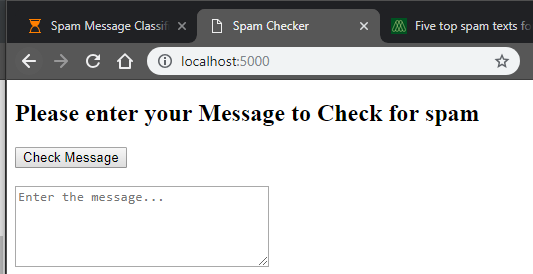
\includegraphics{images/1.png}
\caption{}
\end{figure}

    \begin{figure}
\centering
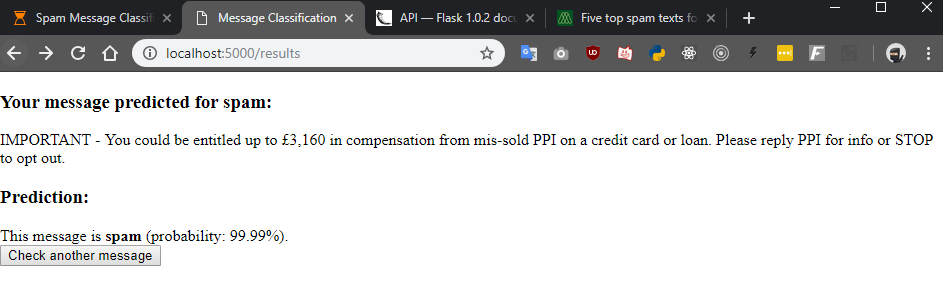
\includegraphics{images/2.png}
\caption{}
\end{figure}

    \begin{figure}
\centering
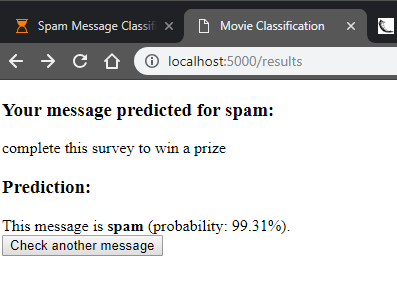
\includegraphics{images/3.png}
\caption{}
\end{figure}

    \begin{figure}
\centering
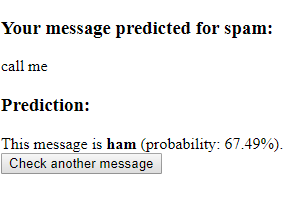
\includegraphics{images/4.png}
\caption{}
\end{figure}


    % Add a bibliography block to the postdoc
    
    
    
    \end{document}
